\section{Results}
\label{sec:results}

\begin{figure}
    \centering
    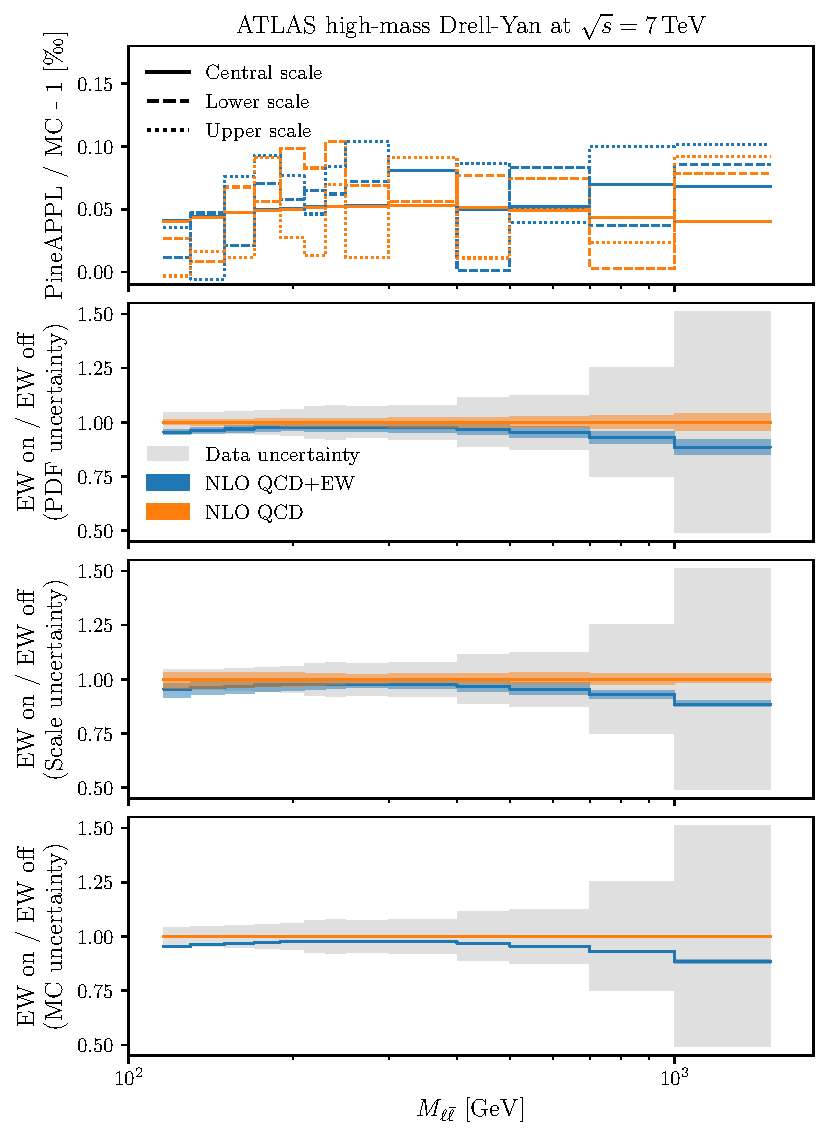
\includegraphics[width=0.5\textwidth]{figures/pineappl_ATLASZHIGHMASS49FB}
    \caption{PineAPPL comparison for ATLAS high-mass Drell-Yan at $\sqrt{s}=7$ TeV.}
    \label{fig:atlaszhighmass49fb}
\end{figure}

\begin{figure}
    \centering
    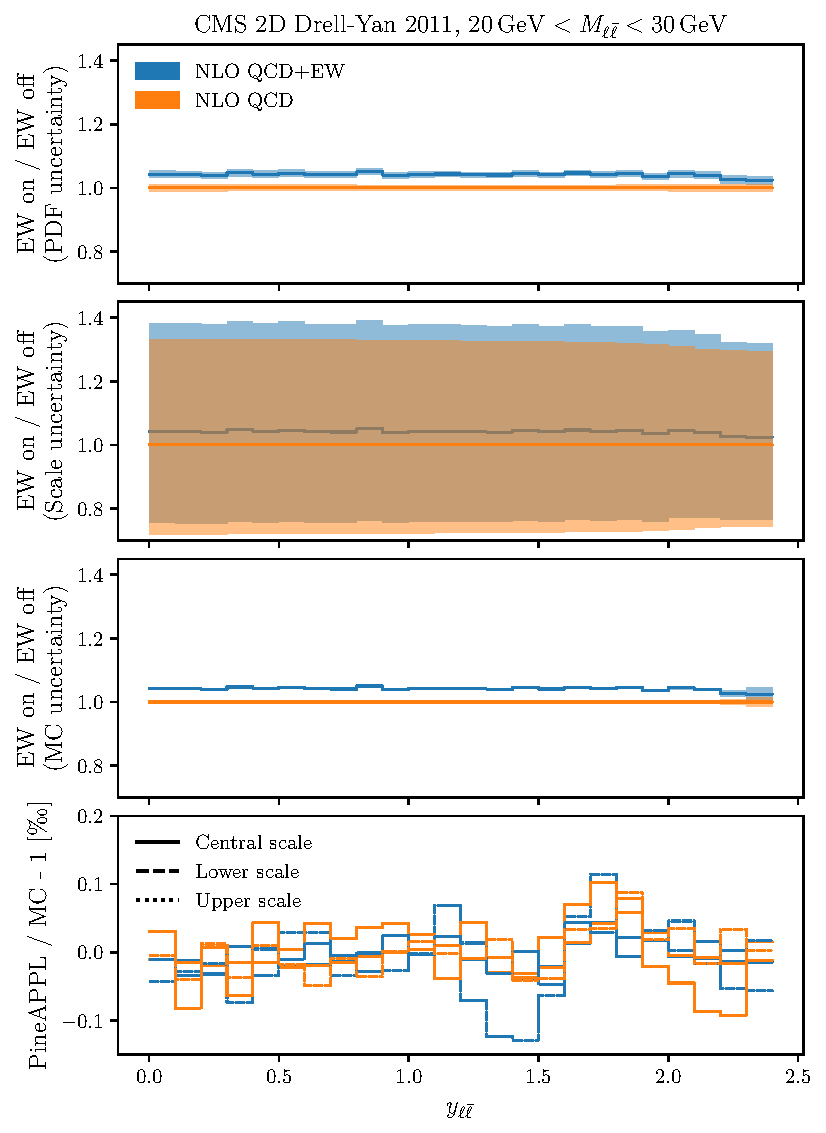
\includegraphics[width=0.5\textwidth]{figures/pineappl_CMSDY2D11_bin1}%
    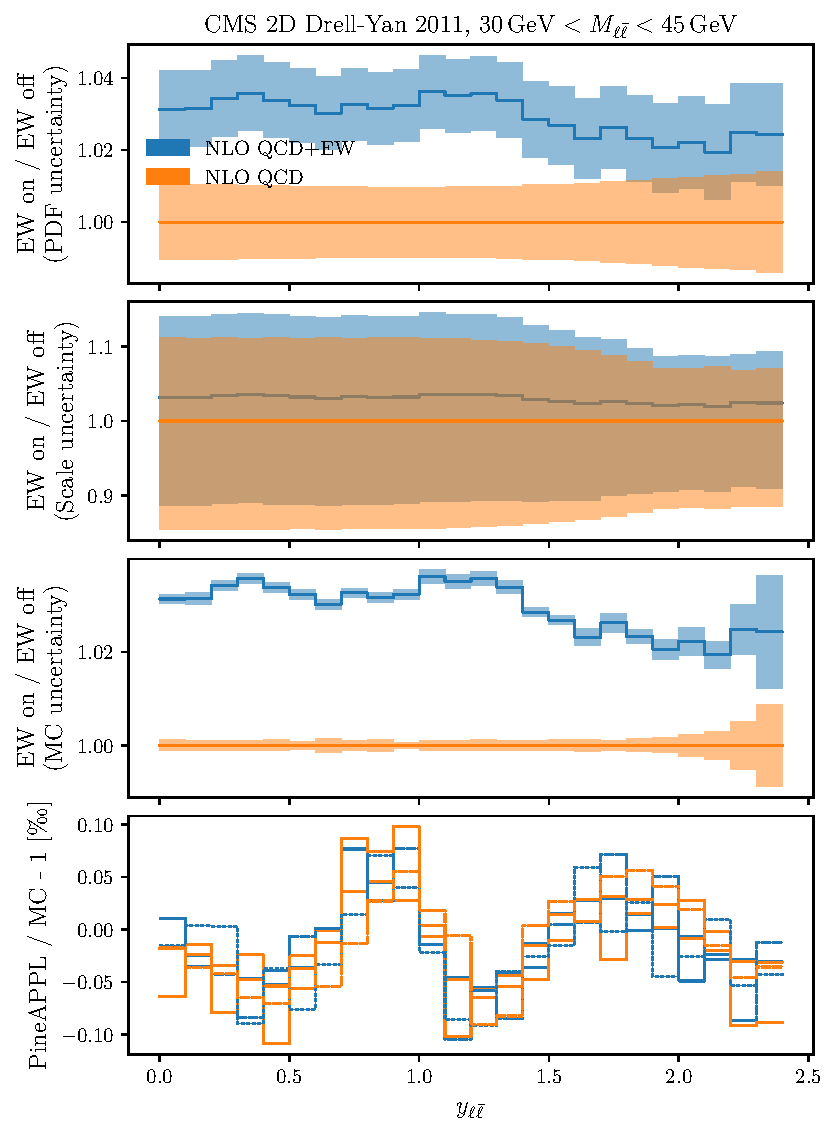
\includegraphics[width=0.5\textwidth]{figures/pineappl_CMSDY2D11_bin2}
    \caption{PineAPPL comparison for CMS 2D Drell-Yan.}
    \label{fig:cmsdy2d11_bins12}
\end{figure}

\begin{figure}
    \centering
    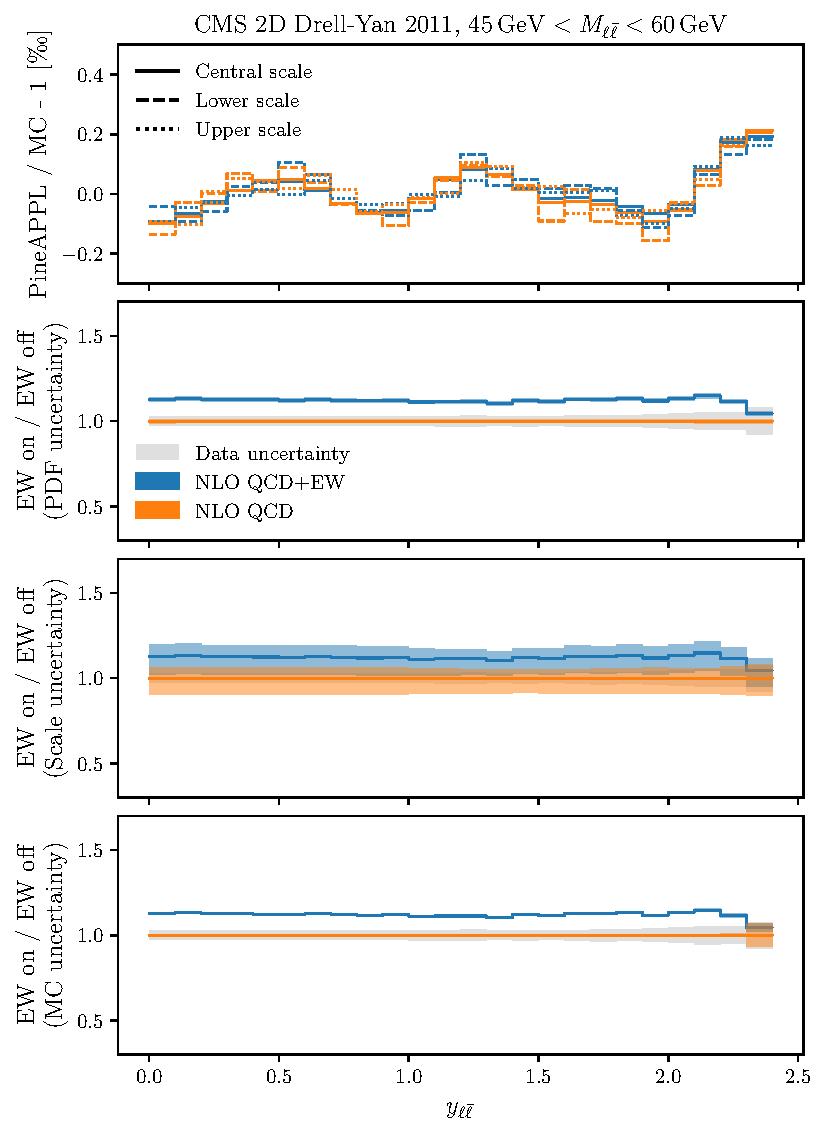
\includegraphics[width=0.5\textwidth]{figures/pineappl_CMSDY2D11_bin3}%
    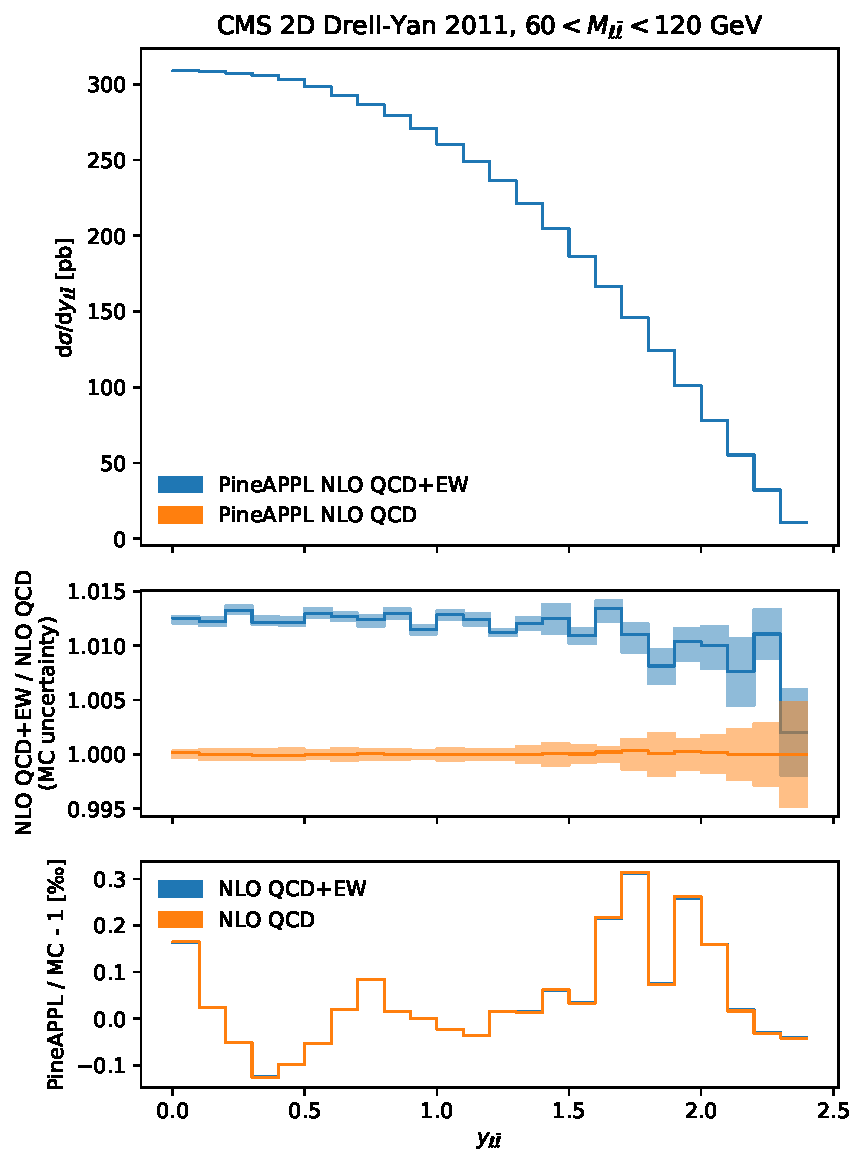
\includegraphics[width=0.5\textwidth]{figures/pineappl_CMSDY2D11_bin4}
    \caption{PineAPPL comparison for CMS 2D Drell-Yan.}
    \label{fig:cmsdy2d11_bins34}
\end{figure}


\begin{figure}
    \centering
    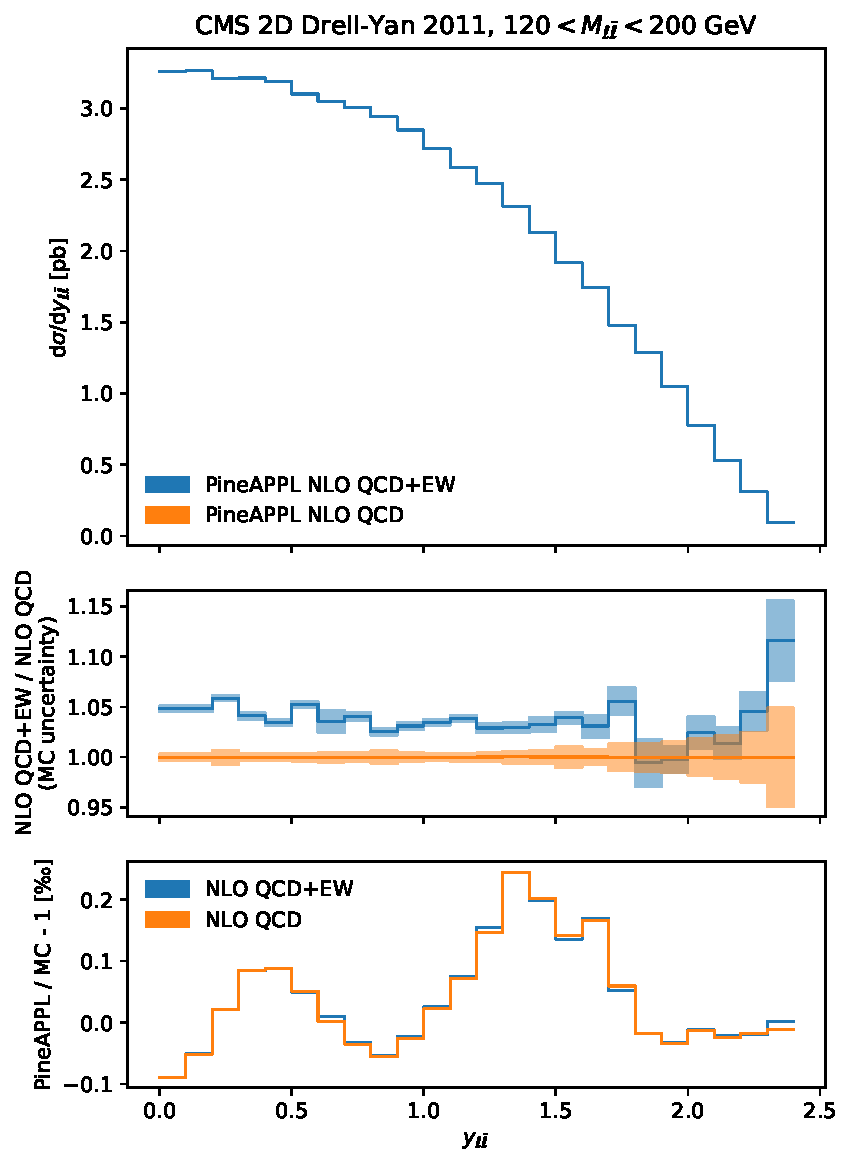
\includegraphics[width=0.5\textwidth]{figures/pineappl_CMSDY2D11_bin5}%
    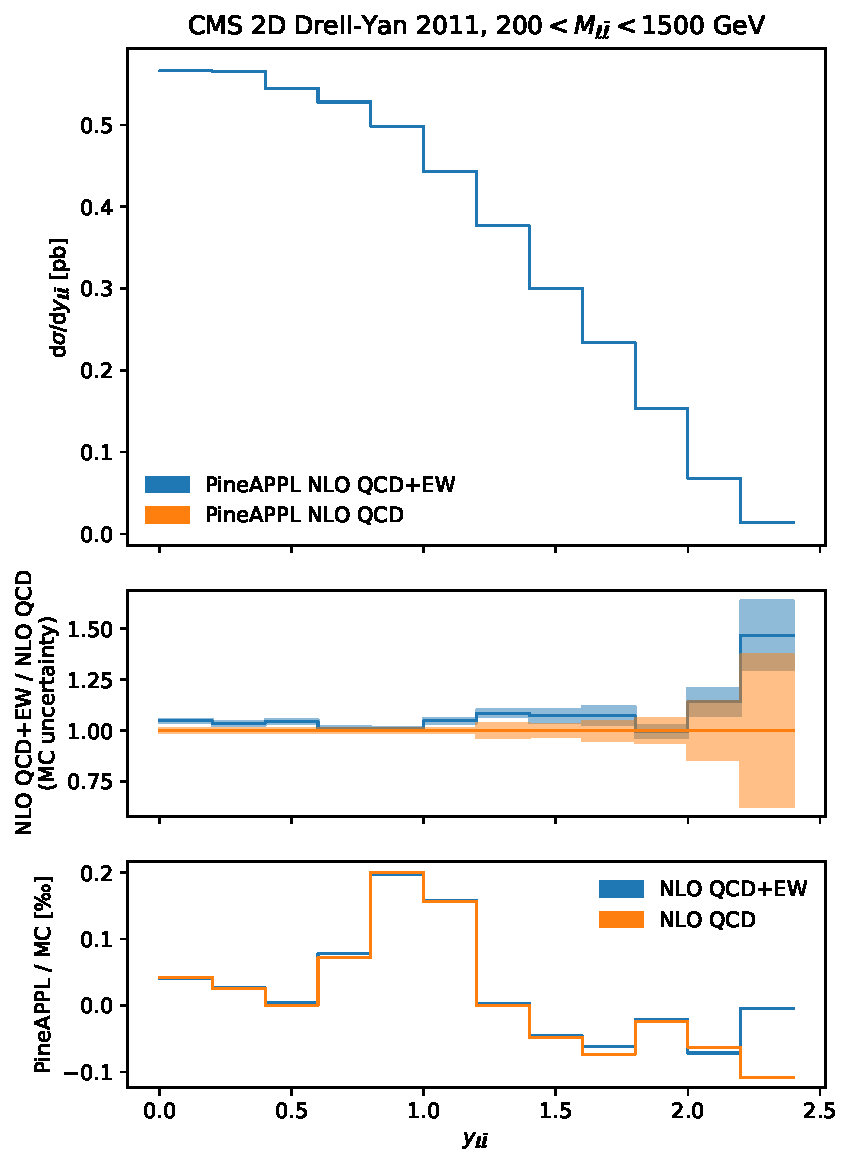
\includegraphics[width=0.5\textwidth]{figures/pineappl_CMSDY2D11_bin6}
    \caption{PineAPPL comparison for CMS 2D Drell-Yan.}
    \label{fig:cmsdy2d11_bins56}
\end{figure}


ERN 7 Apr: there is consensus on the fact that we should present results for the
following data sets:
\begin{itemize}
\item ATLAS high mass DY distributions, 7 TeV~\cite{Aad:2013iua} (CS);
\item CMS 2D DY distributions, 7 TeV~\cite{Chatrchyan:2013tia} (CS);
\item ATLAS top pair differential distributions ($m_{t\bar{t}}$ and $p_T^t$),
8 TeV~\cite{Aad:2015mbv} (ERN);
\item CMS $Z$ $pT$ distributions, 13 TeV~\cite{Sirunyan:2019bzr} (ERN).
\end{itemize}

We agree not to display any LHCb measurement, given that they won't add
further value to our discussion.
Note added: we might also want to have a look at the ATLAS 2D and 3D DY
distributions, 8 TeV~\cite{Aad:2016zzw,Aaboud:2017ffb}, if time allows
us to do so.

CS 25 Jun: We've agreed to show basically two types of plots: 1) technical plots showing the good agreement between the MC compared to the results from the grids, and 2) phenomenological results showing larger EW corrections, for example.
In the aMCfast paper both is shown in single plot, but since we have more to show, I suggest the following: for the technical plots we show a 2x2 matrix of plots, each showing the difference of the grid result compared to the MC result, in the following fashion:
\begin{itemize}
\item NLO QCD with low statistics,
\item NLO QCD+EW with low statistics,
\item NLO QCD with high statistics, and finally
\item NLO QCD+EW with high statistics,
\end{itemize}
each showing a few scale variations.
These plots then clearly show that no matter what corrections you choose, no matter the statistics, and no matter the scale variation, the agreement is always excellent.
In any case I would like to avoid showing a plot with absolute numbers and low statistics, which looks a bit ridiculous in my opinion (look at figure 1, left side, top plot of the aMCfast paper).

Finally we can show another series of plots, which in my opinion should be very similar to the usual pheno paper plots: absolute numbers with a scale variation band, maybe a few corrections shown in the same plot and then in the bottom relative corrections.
